
   \chapter{Gestion de Projet}
   \minitoc
      \section{Généralités}
      Ce projet se développe dans le cadre du module du P2II, il vise la mobilisation des connaissances acquises durant les différents modules de l'année scolaire, y compris la Gestion de Projet. \\
      
      Les algorithmes et leur étude développés lors de ce projet doivent répondre à l’énoncé fourni par Sébastien Da Silva et Gérald Oster. Tous les élèves participant au projet doivent travailler dans le déroulement de chacune de ses parties, autant comme développeurs que managers. Le projet s'est déroulé suivant le principe de la méthode Agile.\\


      \section{Outils de gestion de projet}
      \textit{Le bon outil pour le bon usage}.\\
      
      Pour bien gérer notre projet et pour respecter les consignes de l'énoncé, nous nous sommes appuyés sur plusieurs outils de gestion de projet:\\
      
      \begin{itemize}
         \item Charte de projet 
         \item Matrice SWOT
         \item Matrice RACI 
         \item Comptes-rendus rédigés lors de chaque réunion 
         \item Méthode Agile
      \end{itemize}
      
         \subsection{Charte de projet}
            
            \begin{itemize}
                \item {\textbf {Cadrage/Finalités et importance du projet}} \\
               \\
                
                \item {\textbf {Objectifs et résultats opérationnels}}\\
                

Tous les élèves participant au projet doivent maîtriser les différentes parties de l’application de tel sorte qu’ils soient capables de répondre à des questions sur ces dernières. Le projet se déroule par jalons définis à partir des sous-parties de l’énoncé.\\

Le projet vise à livrer une application, incluant une base de données et une méthode d’insertion de données depuis des fichiers excel et csv, qui sera notée.
Le projet cherche à répondre à la totalité des questions de son énoncé. On s’intéresse à la création d’une application qui permet l’utilisation et la modification d’une base de données créée à partir de fichiers fournis. Le développement et l’étude des fonctions algorithmiques, l’application résultante ainsi que la gestion du projet seront conçus par touts les participants et le compte-rendu final comportera un document rédigé sur Latex ainsi qu’une présentation orale accompagnée d’une démonstration. À l’issue du compte-rendu, le module sera soumis à une validation.  
\\


                
                \item {\textbf {Déroulement du projet/Organisation/ressources}}\\
                \begin{itemize}
                    \item Dans le déroulement de ce projet, les participants sont :\\
                    
                    LEDEUX Flavien\\
                    ROURA Guilhèm\\
                    ZHU Céline\\
                   
                    
                    Chacun des membres du groupe ont le même rôle en tant que développeur et manager.\\
                     \item Les moyens à disposition sont multiples :\\
                    - Logiciels de traitement de texte tel Latex\\
                    - Logiciels permettant travaille en équipe tel Gitlab\\
                    - Connaissances acquises lors de l'année scolaire 2020-2021 à TELECOM Nancy pour le développement et l’étude d’algorithmes\\
                    - Connaissances acquises lors du module de MOOC-GdP pour la gestion de projet\\
                    - Éventuelle aide des professeurs de TÉLÉCOM Nancy\\
                \end{itemize}
                \item {\textbf {Jalons : échéancier / événements importants}}\\
                
                 \begin{center}
         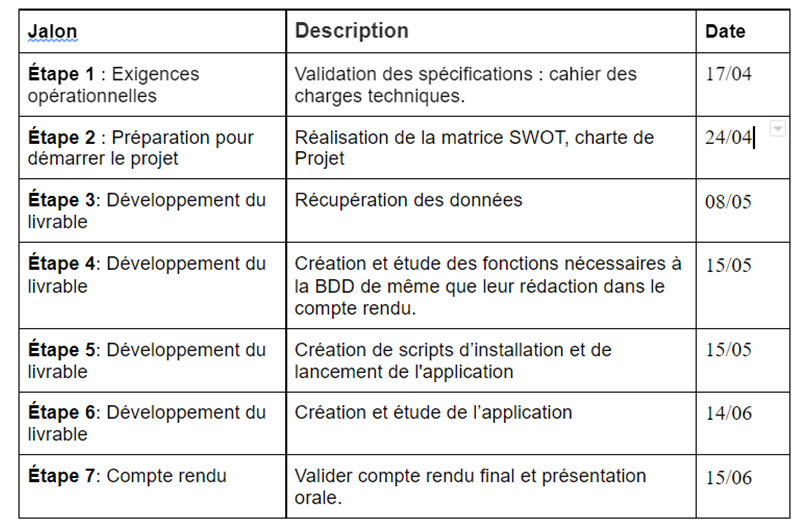
\includegraphics[width=15cm]{jalons.png}\\

         \end{center}

                \item {\textbf {Risques et opportunités}}\\
                Après analyse du déroulement du projet, on dégage:\\
                
                \qquad Plusieurs risques tels: \\
 - Un potentiel mauvais accès à internet\\
- Une absence de date butoir\\
- Le sujet n’est pas entièrement défini\\


	            \qquad Plusieurs opportunités telles:\\
-La possibilité de solliciter une personne extérieure au projet pour s'entraîner à la présentation orale\\

-La possibilité de demander de l'aide à un professeur en cas de blocage\\

-Accès à l’école et à son matériel\\
-Beaucoup de documentations en ligne\\

                 
                \end{itemize}   
                
            
                
            \subsection{Matrice SWOT}
    
                
                 \begin{center}
         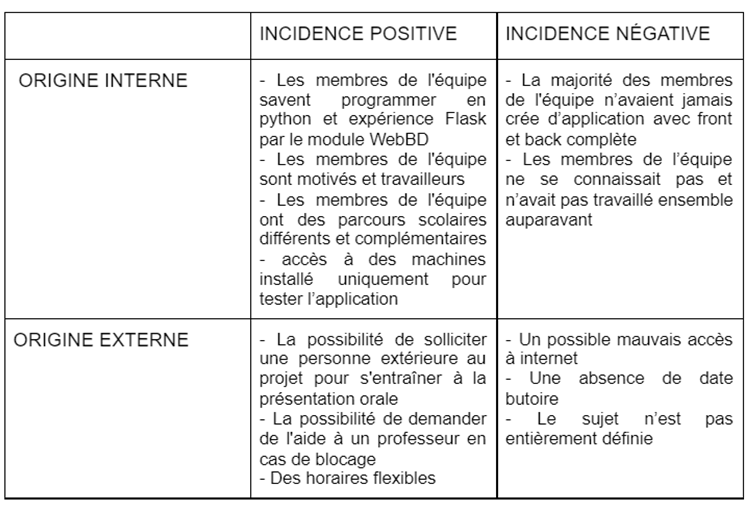
\includegraphics[width=15cm]{swot.png}\\

         \end{center}
    

         
        
        \subsection{Matrice RACI}
        
        Nous avons réalisé une matrice RACI dans le but de formaliser le rôle de chacun lors des différents lots de travail et avoir une idée claire de nos responsabilités. 
        
        La matrice RACI est illustrée par la figure ci-dessus.
         
       \subsection{Méthode Agile}
       En ingénierie informatique, la méthode Agile se base sur un cercle vertueux d'auto-discipline centrée sur la confiance en autrui et sur un feedback régulier. Nous avons décidé d'utiliser cette méthode plutôt que la méthode linéaire traditionnelle, car la méthode Agile permet des réponses très flexibles aux changements et aux imprévus. Étant donné la liberté donnée par le sujet, et le problème ouvert, nous avons donc décidé de ne pas s'embarquer dans une méthode trop rigide (Diagramme de Gantt), dans la situation où une grande modification du sujet ait lieux. Néanmoins, afin de se fixer une structure dans notre organisation, nous avons tout de même imposé des réunions dits de "vérification d'avancement". Ce sont des réunions non de travail, mais d'observation de l'avancement de l'équipe ainsi que de partage des difficultés rencontrées. Ces réunions ont donc été fixées à moins d'une heure et cette contrainte a été bien respectée à l'exception de deux réunions. Elle ont été plus focalisés sur la création de documents de gestion de projet.
        \subsection{Comptes-rendus}
        
        À l’issue de chaque réunion, un compte-rendu était rédigé pour résumer les propos traités, formaliser les décisions prises et la liste des responsabilités désignées à chaque membre de l’équipe pour la prochaine réunion. Sa rédaction était prise en charge par chacun d’entre nous de manière cyclique.

Chaque compte-rendu a été rédigé d'après le modèle donnée ci-dessous,la totalité des compte-rendus peuvent être retrouvés dans l'Annexe et sur le dépôt GitLab:
\title{P2II 1A - Compte-rendu n°1}
\begin{center}
        \begin{tabular}{|l|l|}
        \hline
   
\textbf{Motif de la réunion :}&\textbf{Lieu de la réunion :}\\

Réunion de démarrage du projet&Réunion en visioconférence sur Discord\\


        \hline
        \textbf{Présents :}&\\

Flavien LEDEUX&\textbf{Date :} 03/04/2021\\

Guilhèm ROURA&\\
Céline ZHU&\textbf{Heure :} 10h01\\

&\\
\textbf{Absent :}&\textbf{Durée :} 45 minutes\\

Personne&\\
&\\
\textbf{Rédaction du compte-rendu :}&\\

Céline ZHU&\\

        \hline
        \end{tabular}\\
        \end{center}
\minitoc


\section{Prendre connaissance du sujet}

Rapport sur la Gdp et la réflexion\\
    Objets à rendre:\\
    Base de données SQL standard + schéma\\
    Rapports formats html ( rédigé en fonction de quoi à demander à M Da silva ou M Oster)\\
Afficher les résultats des requêtes que ce soit en schéma ou par texte\\
L’état des fichiers final ou pas.\\
\section{Établir les outils de GdP}
Fichier Readme.md\\
Matrice RACI\\
Gantt \\
SWOT\\
\section{Établir le Cahier des charges}
Base de données SQL:\\
script Python rendant une base de données cohérente\\
Avec des informations\\
Trois étapes: Design, construction, tests boîte noire/blanche\\
	  - Application Python ( html):\\
			- Tous Flask\\
			- Définir tous les liens qui sont liés à notre application\\
			- Définir les conventions Html\\
			- Fiches de style\\
\section{Latex (?)}
Création du latex sur Overleaf et séparation en plusieurs fichiers Tex plus tard.\\
Programmation\\
 Flavien:  Python(flask) et Sqlite sont plus pratiques pour des amateurs. et on peut s’aider de la WebBD.\\

\section{ Planifier la semaine d'après }
	- Faire les scripts de la base de données pour les créer et le schéma.\\
		- Schéma: Flavien/Guilhèm\\
		- Scripts: Céline\\
		- Tests: Flavien/Céline\\
	-Commencer à réaliser les classes représentant les différentes éléments à ajouter dans la BDD.\\
	- Documenter vos actions en latex.\\
Prochaine réunion:\\
Samedi à 10h01 10/04/21:\\
	odj: \\
- Avancement du projet\\
	- Construction de la matrice RACI\\
	- Faire le Gantt\\
	- Dire les endroits qui nous ont posés problèmes\\


      \section{Organigramme projet}
      
      Selon leur localisation dans l'organigramme, il existe 3 types de projets:
      
      \begin{itemize}
          \item Au sein d'un même service: c'est un \textit{projet local}.
          \item Impliquant plusieurs services différents: des \textit{projets transversaux}.
          \item \textit{projets sortis}: de taille importante et font appel à des intervenants détachés spécialement.
      \end{itemize}
      
      Notre projet est clairement un projet transversal au sein d'une structure fonctionnelle.
      
      En effet, la structure fonctionnelle est une structure où il n'y a pas de chef de projet, ce qui encourage l'initiative, favorise l'adaptation aux évolutions de l'environnement et facilite la circulation des informations. De plus, la division du travail se fait par fonctions ce qui favorise l'efficacité du travail.
      
      Cette structure a permis à chacun d'entre nous de décider quelles tâches leur a été confiées:
      
      \begin{itemize}
          \item \textbf{Flavien Ledeux}
          \begin{itemize}[label=$\bullet$]
              \item réalisation des script de création de la base de données (BDDCreation.py)
              \item réalisation du script d'upload des données vers la base de données depuis un répertoire (ImportRepository.py)
              \item réalisation des script d'installation automatique installer (Windows et Linux)
              \item mise en place du polymorphisme sur les fonctions de lecture de fichier et création d'une fonction l'utilisant pour retourner les informations du fichier
              
              \item création des tables notes, voeux\_ecole et ranginfo ainsi que les tables qui dépendent de ces dernières
              \item mise a jour et correction du schéma de la base de données
              
              \item Réalisation des fonctions Add sous leur forme initial
              \item réalisation des fonctions qui insèrent des informations vers la base de données sauf pour les fichiers inscription et listeEtablissement (\ref{tab:TableKeyChar} page \pageref{tab:TableKeyChar})
          \end{itemize}
          
          \item \textbf{Guilhèm Roura}
          \begin{itemize}[label=$\bullet$] 
              \item Réalisation d'une partie du schéma de la BDD, notamment la table candidat.
              \item Réalisation de l'insertion des données provenant du fichier Inscription.
              \item Fonction d'insertion dans la BDD (\textit{InsertData} et \textit{InsertOrUpdateData})
              \item Modification des fonctions Add pour supprimer le redondance du code d'insertion des tables, en utilisant les 2 fonctions ci-dessus
              \item Fonction de statistiques et de test.
              \item Relecture et corrections diverses dans les différentes fonctions
              
          \end{itemize}    
          \item \textbf{Céline Zhu}: 
                \begin{itemize}[label=$\bullet$] 
              \item Réalisation d'une partie du schéma de la BDD, notamment la création des tables adjacentes à la table candidats et de leurs jointures
              \item réalisation des scripts de lecture des fichiers Excel et CSV
              \item réalisation de la fonction d'upload des données pour listeEtablissement
              \item réalisation de l'application Flask
              \item réalisation des fichier .sh pour automatiser Flask et automatiser la création de l'environnement virtuel nécessaire
          \end{itemize}
      \end{itemize}
      
      
      